\subsection{Dwarf Galaxies as Lenses \Contact{Yao}}
\Contributors{Yao, Annika, James, Tony, Manoj?, ...}
\label{sec:halo_profile_group}

%\ADW{I think we need to make it clear early on that we are talking about dwarfs beyond the Local Group.}
%\ADW{I think that the structure of this section could be: (1) intro to the core-cusp problem (more focus than missing satellites), (2) description of the LSST lensing projections, (3) connect back to dark matter physics (i.e., how will a lensing signal help us solve cusp/core.}

Dwarf galaxies ($M_\star \lesssim 10^{9} \Msun$) provide the best visible tracers of low-mass dark matter halos. 
The relatively low baryonic content makes dwarf galaxies sensitive probes of  dark matter physics through the shape of their dark matter halo profiles. 
In particular, the ``core-cusp'' problem in dwarf galaxies has been cited as one of the most significant challenges to CDM \citep[\eg,][]{2010AdAst2010E...5D,Bullock:2017xww}.
The standard CDM model predicts that dark matter halos should have steeply rising (``cuspy'') central densities in contrast to the shallower (``cored'') mass profiles that are observationally inferred for many dwarf galaxies.  
Evidence for cored profiles exists for Milky Way satellite galaxies from kinematic and theoretical studies \citep[\eg][]{Walker:2009, 2012ApJ...759L..42P}, and is stronger when one studies the inner density profiles of dwarf galaxies based on high-resolution neutral hydrogen surveys \citep[\eg][]{Begum:2008,Hunter:2012,Cannon:2011,Oh:2015}. 
Many of these observations show inferred central slopes of the dark matter density profile, $\rho(r) \sim r^{\gamma}$, that are significantly shallower ($\gamma \approx 0$--$0.5$) than the CDM prediction $\gamma \approx 0.8$--1.4 \citep{Navarro:2010}.

A wide range of solutions to the core-cusp problem have been proposed including observational, astrophysical, and dark matter explanations.
From a dark matter perspective, SIDM can significantly suppress the the central density of halos.
A self-interaction cross-section of $\sigma / m \sim 1 \cm^2 \g^{-1}$ can explain the diversity of rotation curves seen in low-mass spiral galaxies \citep[\eg][]{1504.01437,2017PhRvL.119k1102K,1705.02358}.
In addition, ultra-light or fuzzy dark matter has also been suggested as a possible solution to the core-cusp problem through the formation of uniform density solitonic cores \citep[\eg][]{1502.03456,Hui:2017}. 
However, baryonic feedback remains as a major source of complication for interpreting central density profile measurements in a dark matter context \citep{Madau:2014,Read:2016}. 
If dwarf galaxies form enough stars, energy from SN explosions can flatten the profiles of dark matter and baryons; however, if too many stars are formed, they can have the opposite effect because of the excess baryonic mass steepening the slope of the central density profile \citep{Bullock:2017}.
Technical challenges in implementing multi-phase gas and baryonic physics make it difficult to directly address and calibrate baryonic predictions based on hydrodynamical simulations \citep{Tollet:2016,1611.02281,Sawala:2016}.
However, one key prediction is that the creation of cores will be sensitive to the exact star formation rate \citep[\eg][]{governato2012,dicintio2014,onorbe2015,Read:2016,read2018}.
Thus, robust measurements of both the stellar and dark matter mass of dwarf galaxies is essential to investigate the effect of baryonic feedback on the central dark matter density.
%It has been argued that observational and astrophysical systematics, such as beam smearing, center offsets, inclinations, and non-circular motions can bias central density measurements toward flatter profiles \citep[\eg][]{astro-ph/0006048,2004ApJ...617.1059R,2008AJ....136.2761O}. 

LSST can provide a joint statistical measurements of both the central density and stellar content of dwarf galaxies. 
The stacked gravitational weak lensing signal from a large sample of dwarf galaxies will provide the most direct measurement of the amount and distribution of dark matter.  
In this section we make a prediction of LSST's sensitivity to a stacked weak lensing signal from dwarf galaxies.

\paragraph{Dwarf galaxy lenses}
We are interested in estimating the number of isolated dwarf galaxies accessible to LSST as a function of dark matter halo mass.
To predict the abundance of the dwarf  galaxy sample, we assume the mass-to-light ratio derived from the subhalo abundance matching and the global galaxy luminosity function
 \citep{2015MNRAS.451.1540L}.
We use this predicted galaxy luminosity to estimate the limiting redshift for dwarf galaxy detection as a function of galaxy halo mass for two LSST limiting magnitudes: $r \sim 25$ and $r \sim 27$. 
\figref{dwarf_redshift} shows that to probe dark matter halos with mass $\lesssim 10^9 \Msun$, it will be necessary to select galaxies at $z < 0.01$. 
While selecting very low-$z$ galaxies with photometric data is challenging, current projects like the SAGA Survey \citep{Geha:2017} have shown that it is possible using data from SDSS. 
DESI and other  future large, multi-object spectrographs will greatly expand the spectroscopic data for training these selections. 
It will also be possible to use morphological information to select nearby dwarf galaxies.
LSST will be able to distinguish a dwarf galaxy with $M_V=-14$ from background galaxies of the same apparent magnitude out to a distance of $\roughly 100 \Mpc$ \citep[Section 9 of][]{0912.0201}.

\begin{figure}
\centering
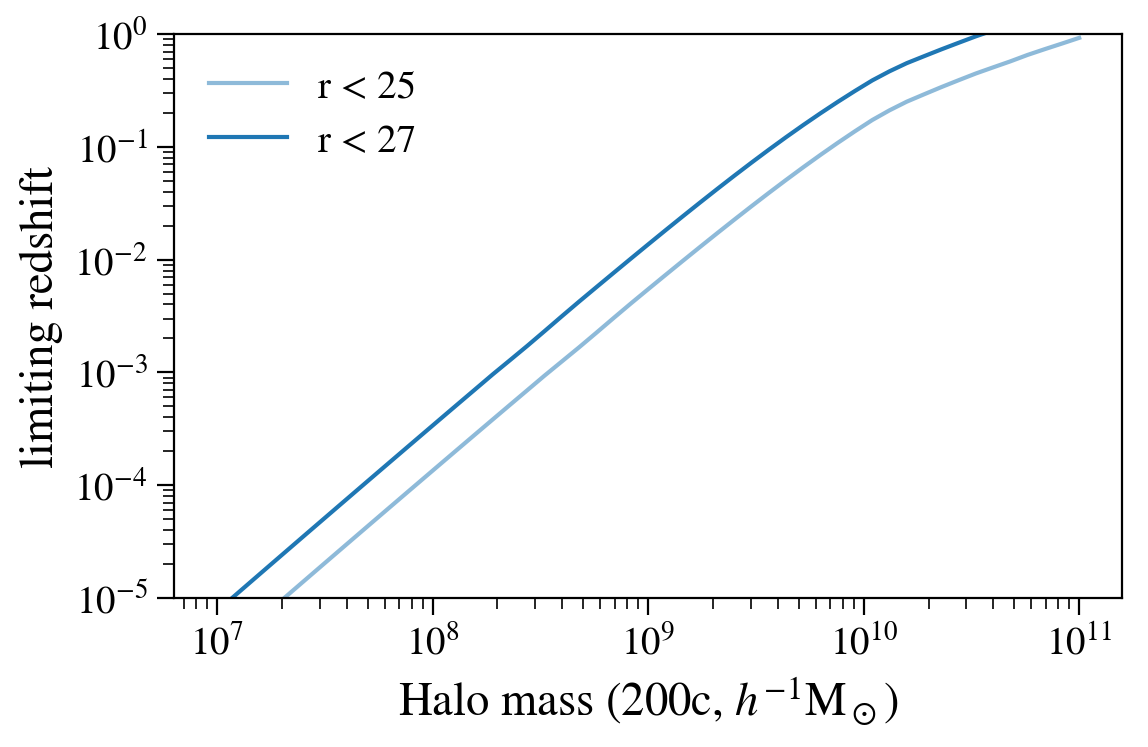
\includegraphics[width=0.7\columnwidth]{halo_mass_redshift_log}
\caption{\label{fig:dwarf_redshift} Limiting redshift for detecting a dwarf galaxy that lives in a dark matter halo of certain masses, assuming a luminosity--halo mass relation from abundance matching.}
\end{figure}


\paragraph{Source galaxies}
The conservative LSST 10-year ``gold'' sample for cosmic shear measurements of dark energy is expected to have a source galaxy density of $\roughly 27 \amin^2$ \citep{Chang:2013,1809.01669}. 
However, we expect that the dwarf lensing analysis can retain significantly more source galaxies for the following reasons.
(1) Our measurement uncertainty is dominated by the low number of dwarf galaxy lenses, rather than the  multiplicative shear measurement bias that must be strictly controlled for dark energy measurements. This allows us to include fainter, smaller, and more blended sources.
(2) Unlike the lenses used for cosmic shear measurements, the dwarf galaxy lenses are at very low redshift. This means that most detected sources are background galaxies.
(3) We expect to be able to combine shape measurements from multiple filters, which could increase the source density by $\roughly 80\%$. 
Combining these factors, we estimate a source galaxy density of $50 \amin^2$, which is consistent with the fiducial, multi-band estimate of \citet{Chang:2013}.
The primary focus of the source galaxy selection will be to avoid catastrophic \photoz outliers (low-$z$ galaxies reported at high-$z$), which are typically less than a few percent in current surveys \citep{1406.4407}. 
%\Photoz algorithms incorporating machine learning currently achieve better performance, giving posterior p(z) estimating which enables cuts on suspect source galaxies. 

\paragraph{Sensitivity}
We calculate the expected strength of a lensing signal for three different bins in halo mass,  $M = \{10^{10} \Msun, 3\times10^9 \Msun, 10^{9} \Msun \}$, each with a width of $0.5$\,dex in mass. 
These samples corresponds to $N = \{1.2\times10^8, 7.8\times10^6, 1.6\times10^5\}$ dwarf galaxies out to a redshift of $z = \{0.35, 0.07, 0.014\}$, respectively.
Source galaxies are placed at $z = 1.2$ with a density of $50 \hbox{ arcmin}^{-2}$ and a shear uncertainty of $\sigma_\gamma = 0.25$.
We model the mass distribution in each dwarf galaxy with an NFW halo assuming the concentration-mass relationship from \citet{1809.07326}.
We calculate the shear from the stacked dwarf galaxy lens sample using \code{galsim}, assuming that each lens is  placed at the limiting detectable redshift.
The results are shown in \figref{dwarf_sn}, where we find that LSST has the potential to measure the lensing shear with ${\rm S/N} \gtrsim 10$ for halos with $M \gtrsim 3 \times 10^9$.

\ADW{We need to add a projection assuming a cored profile for the lenses. We need a concluding statement to bring this back to the dark matter questions raised in the intro. Should we include some discussion of PSF systematics?}

\begin{figure}
\centering
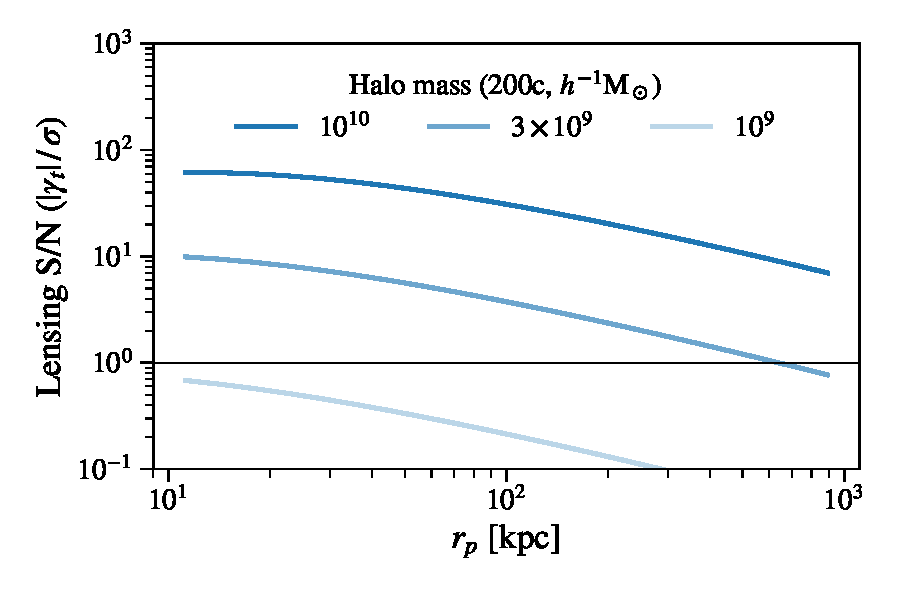
\includegraphics[width=0.7\columnwidth]{halo_mass_lensing_sn}
\caption{
\label{fig:dwarf_sn} Lensing signal-to-noise for stacked samples of dwarf galaxies in three different mass bins with width of 0.5 dex in mass. 
This plot assumes perfect selection of dwarf galaxies within the redshift range over which they are detectable by LSST. 
Source galaxies are assumed to be at $z=1.2$, with a surface number density of $50 \amin^{-2}$, and a shear uncertainty of $\sigma_\gamma = 0.25$ per component.}
\end{figure}

%%%%%%%%%%%%%%%%%%%%%%%%%%%%%%%%%%%%%%%%%%%%%%%%%%%%%%%%%
% ADW: Original text preserved below in a comment block %
%%%%%%%%%%%%%%%%%%%%%%%%%%%%%%%%%%%%%%%%%%%%%%%%%%%%%%%%%

\begin{comment}

Although in general dwarf galaxies mean any ``faint" galaxies, we can broadly classify them
into satellite dwarfs and field (isolated) dwarfs.
Because of non-central terms and two-halo terms, it is difficult to interpret the galaxy-mass correlation measurements of satellite dwarfs. Therefore, isolated dwarf galaxies are the main targets for our dark matter probe using LSST.

\begin{figure}
\centering
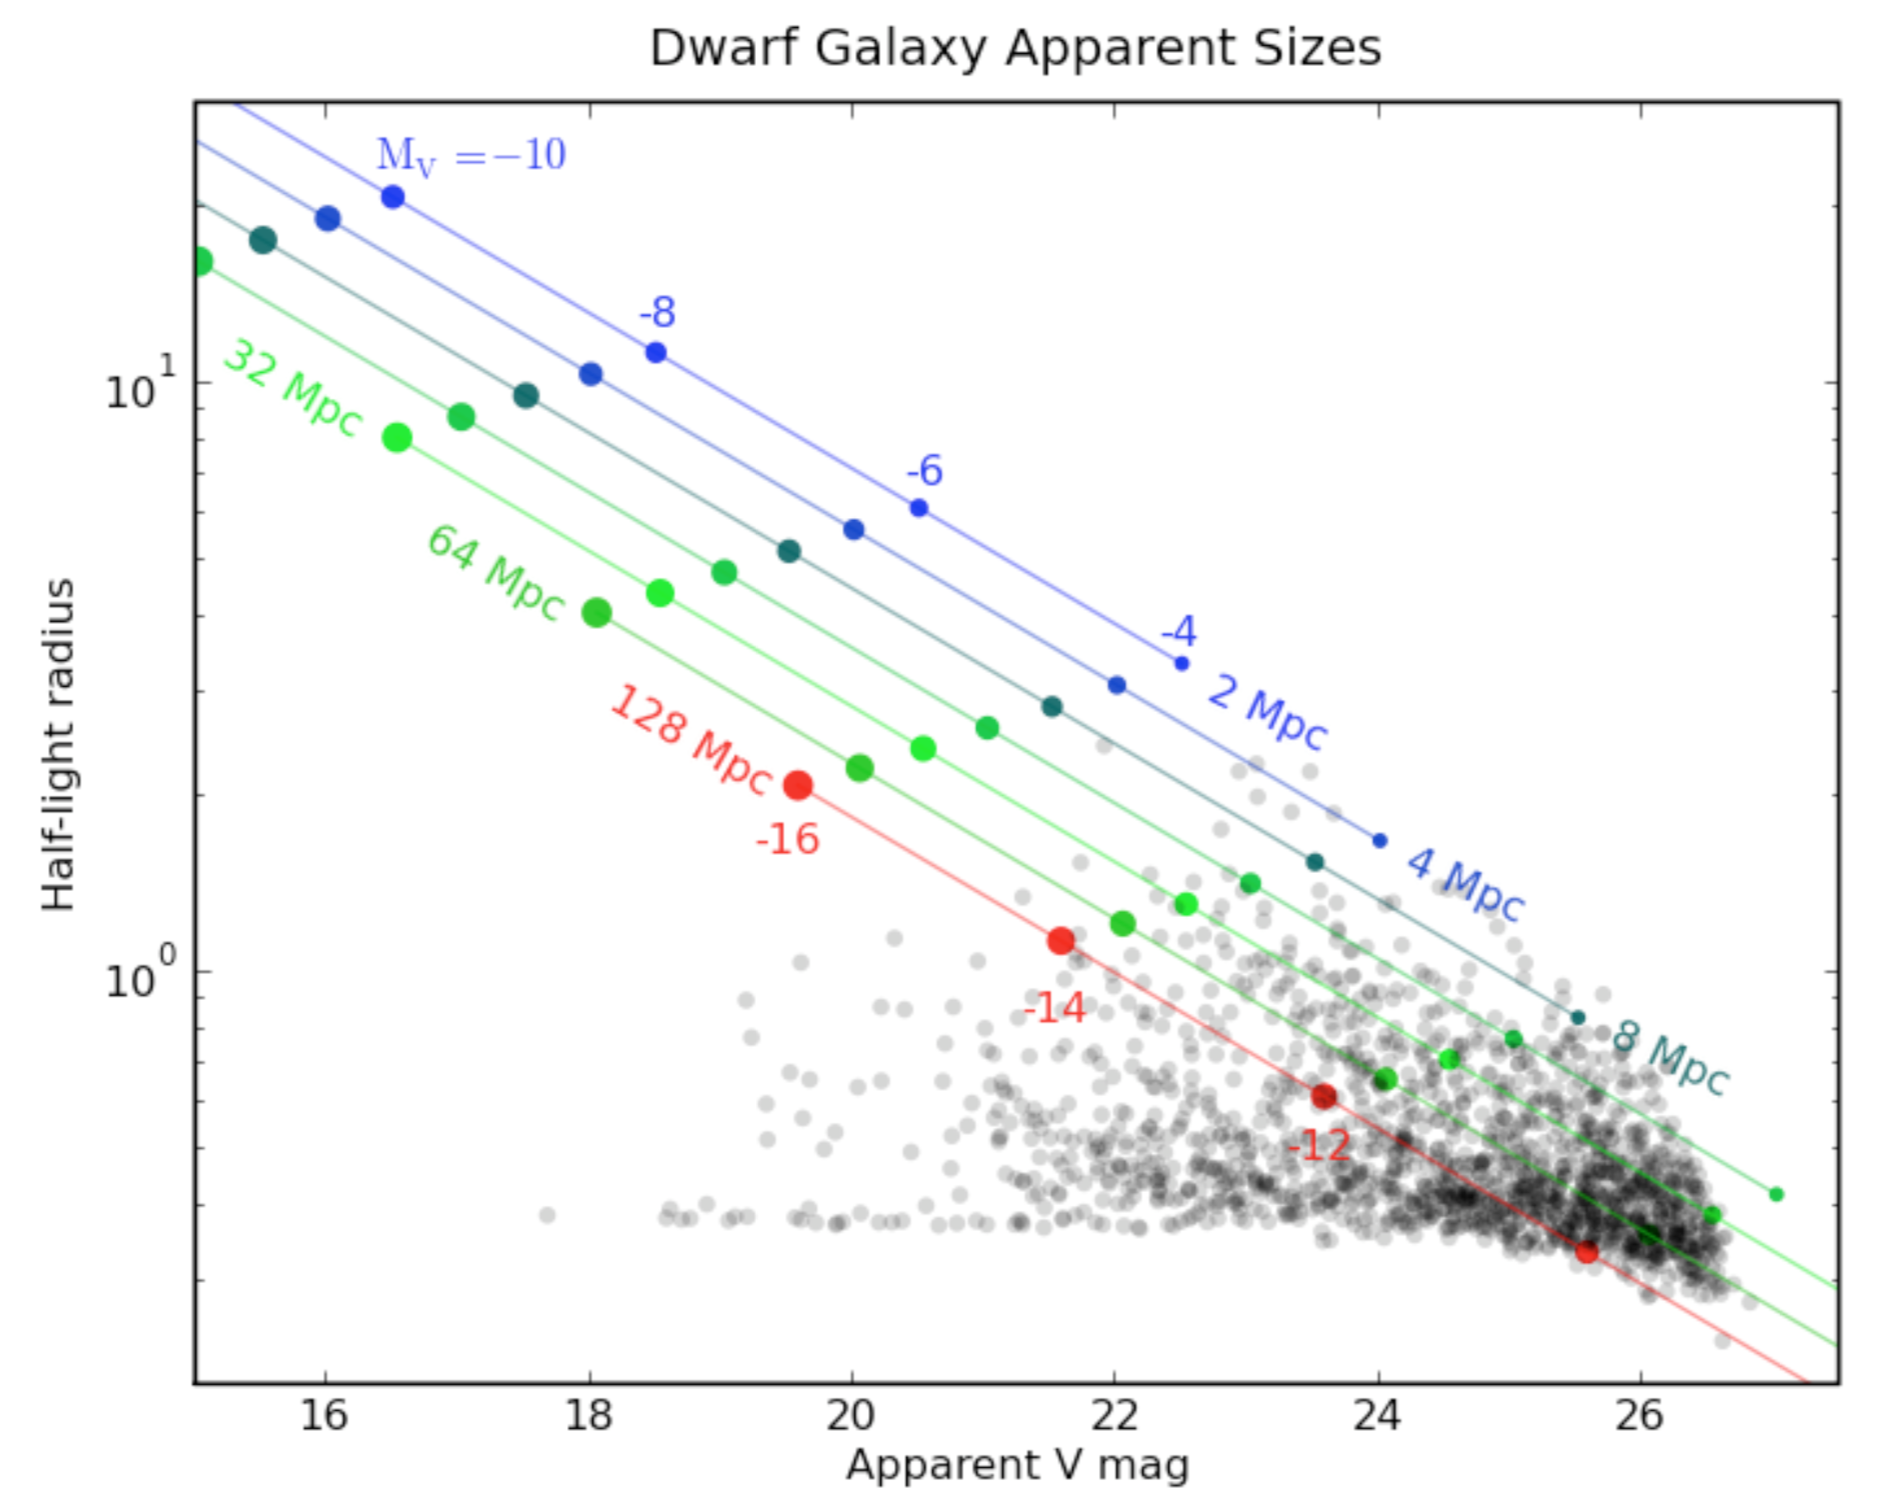
\includegraphics[width=0.6\columnwidth]{dwarf_size.png}
\caption{Magnitude-radius relationship for dwarf galaxies observable with LSST \citep[Figure 9.7 in][]{0912.0201}. 
Colored points and lines show the half-light radii in arcsec for dwarf galaxies for distances between 4 and 128 Mpc.
Gray points indicate the typical sizes of background galaxies. 
%A dwarf galaxy with $M_V = -4$ should be visible and distinguishable from the background out to 4 Mpc
A dwarf with $M_V = -14$ at 128 Mpc will be larger than most of the background galaxies of the same apparent magnitude.
}
\label{fig:LSST_dwarf_detectability}
\end{figure}

When the nominal 10-year LSST mission is completed, the final depth will be $r\sim27$ mag (5 $\sigma$). 
\figref{LSST_dwarf_detectability} shows the half-light radii of dwarf galaxies as a function of their apparent $V$-band magnitude. 
We can estimate that at the distance of Coma ($\roughly100\Mpc$) a dwarf with $M_V=-14$ will be larger than most background galaxies of the same apparent magnitude. 
%Even dwarfs as faint as $M_V=-10$ (comparable to the Draco dwarf spheroidal) will have half-light radii of $\roughly4\asec$, which is separable from stars at $r \sim 25.5$.

\begin{figure}
\centering
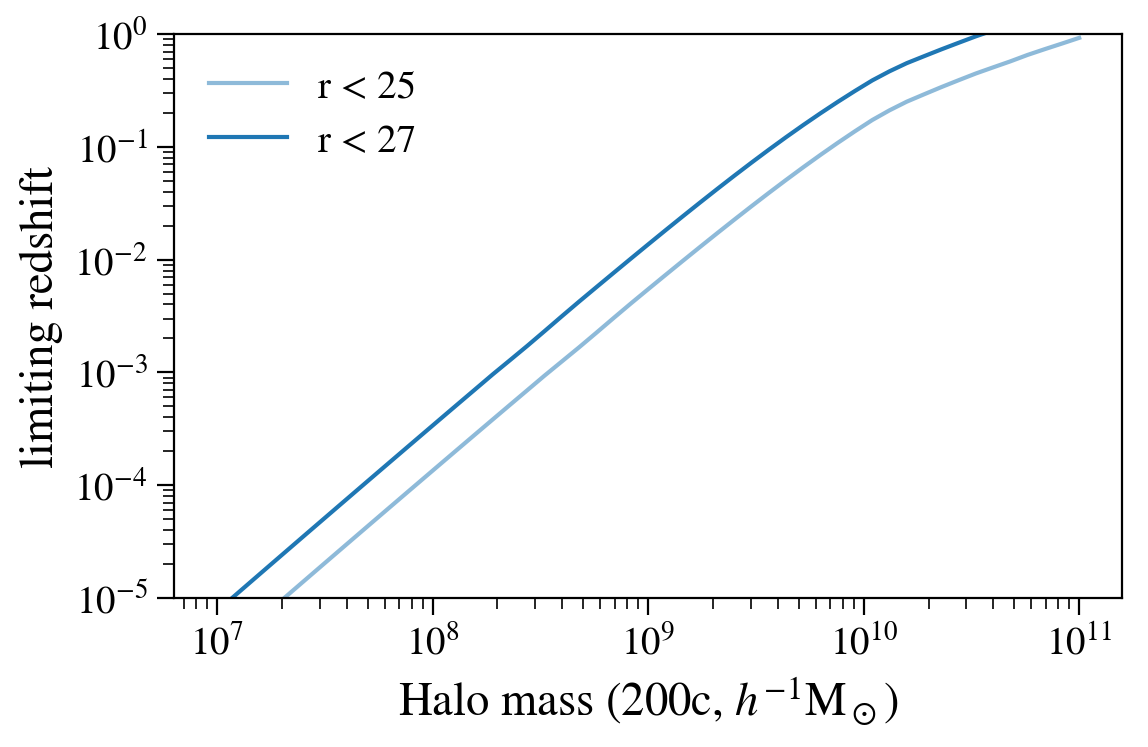
\includegraphics[width=0.7\columnwidth]{halo_mass_redshift_log}
\caption{\label{fig:dwarf_redshift} Limiting redshift for detecting a dwarf galaxy that lives in a dark matter halo of certain masses, assuming a luminosity--halo mass relation from abundance matching.}
\end{figure}

% added by Yao 12/30
Given the LSST detection limit, the redshift range of lens galaxy will depend on the galaxy luminosity, and hence the associated halo mass. 
\figref{dwarf_redshift} shows the limiting redshift for detecting dwarf galaxies as a function of galaxy halo mass assuming two photometric magnitude limits for LSST ($r \sim 25$ and $r \sim 27$). 
The curve assumes a galaxy magnitude--halo mass relation inferred from subhalo abundance matching and a global galaxy luminosity function \citep{1111.0166}. 
In order to probe dark matter halos with mass $\lesssim 10^9 \Msun$ it will be necessary to select galaxies with $z < 0.01$. 

While selecting very low-$z$ galaxies with only photometric data is challenging, it is feasible given advanced target selection strategies and sufficient training data sets. 
For example, the SAGA Survey \citep{Geha:2017} has been searching for low-z satellite galaxies, and its spectroscopic data contain a sample of very low-$z$ galaxy down to a limiting magnitude of SDSS ($r = 21$). 
DESI and other future multi-object spectrographs (i.e., MSE) will also provide new spectroscopic data for training purpose. 

% A few possible strategies:
% 

% LSST detection limit ~ 27
% dwarf galaxy luminosity function
% do we know their size distributions
% how many dwarfs are expected above the LSST detection limit. Maybe a plot showing number of dwarfs vs. magnitude cut.
% isolated vs satellite
% separating true dwarf galaxies from garbage (and from high-z galaxies)
% redshift cutoff

%There are a few possible choices of the combination of redshift and stellar mass (luminosity) of the lens galaxies, with different level of contamination (e.g., photo-$z$ does not do very well below $z<0.1$) and different numbers of available lenses. 

%YYM: Maybe we can have a plot on this? 

\YYM{Here we should discuss how our choices are related to the questions we raised in the first paragraph.}



\paragraph{Constructing source galaxy sample}

The LSST weak lensing Gold sample is expected contain $\roughly 35$ source galaxies per square arcmin. 
However, due to the low redshift of the dwarf galaxy lensing kernel, it is likely that the source galaxy sample can be expanded to include galaxies with less accurate \photoz's.
The primary focus of the source galaxy selection is to avoid galaxies with catastrophic \photoz error (low-$z$ galaxies reported at high-$z$), which is typically less than a few percent in current simulations \ADW{and observations?}. 
%\Photoz algorithms incorporating machine learning currently achieve better performance, giving posterior p(z) estimating which enables cuts on suspect source galaxies. 

\paragraph{Systematic noise floor} PSF systematics set a limit to the weak lens shear floor. The PSF residual systematics in a stack of images of dwarf galaxies of a given mass can be modeled. \figref{psf_systematics} shows the limits attainable by LSST, and  \figref{dwarf_sn} further shows the expected signal-to-noise achievable through a stacked weak lensing analysis of dwarf galaxies depending on host halo mass.

% added by Yao 12/30
In \figref{dwarf_sn}, to calculate the lensing signal, we assume that we are able to select all dwarf galaxies that are detectable by LSST and live halos whose mass is within half dex of the specified mass. All such galaxies are the lens galaxies. For each of the lens galaxies, we assume its host halo has a NFW profile and we stack all their lensing kernels. 
To calculate the noise level, we further assume the source galaxies are all at $z=1.2$, with a surface number density of 50 per squared arcmin, and a shear uncertainty of 0.25 per component. 
We find that we will be able to probe the inner, stacked, dark matter profile ($\sim$ 10 kpc) of halos whose masses are $\sim$ a few times $10^9 M_\odot$ confidently. Of course, the final lens select will likely suffer from incompleteness \YYM{do we want to go into detail on this point?}

Non-cold dark matter models may produce different inner halo profiles; hence, precise measurement of halo profiles, especially of those dark matter dominated systems, provides a new window to probe the nature of dark matter.
In Figure TBD we can see that the two different profiles produce detectable difference in the lensing signal. 
\YYM{We probably need to add a plot to show the difference between two profiles to finish this paragraph...}

% YYM: plot brainstorming: what plot should we include? 
% see some plots that we made last time: 
%https://github.com/lsstdarkmatter/dwarf-halo-mass/tree/master/lensing/plots 
% James Jee: The plot is cool. We can include systematic noise floor into the S/N estimation.

\begin{figure}
\centering
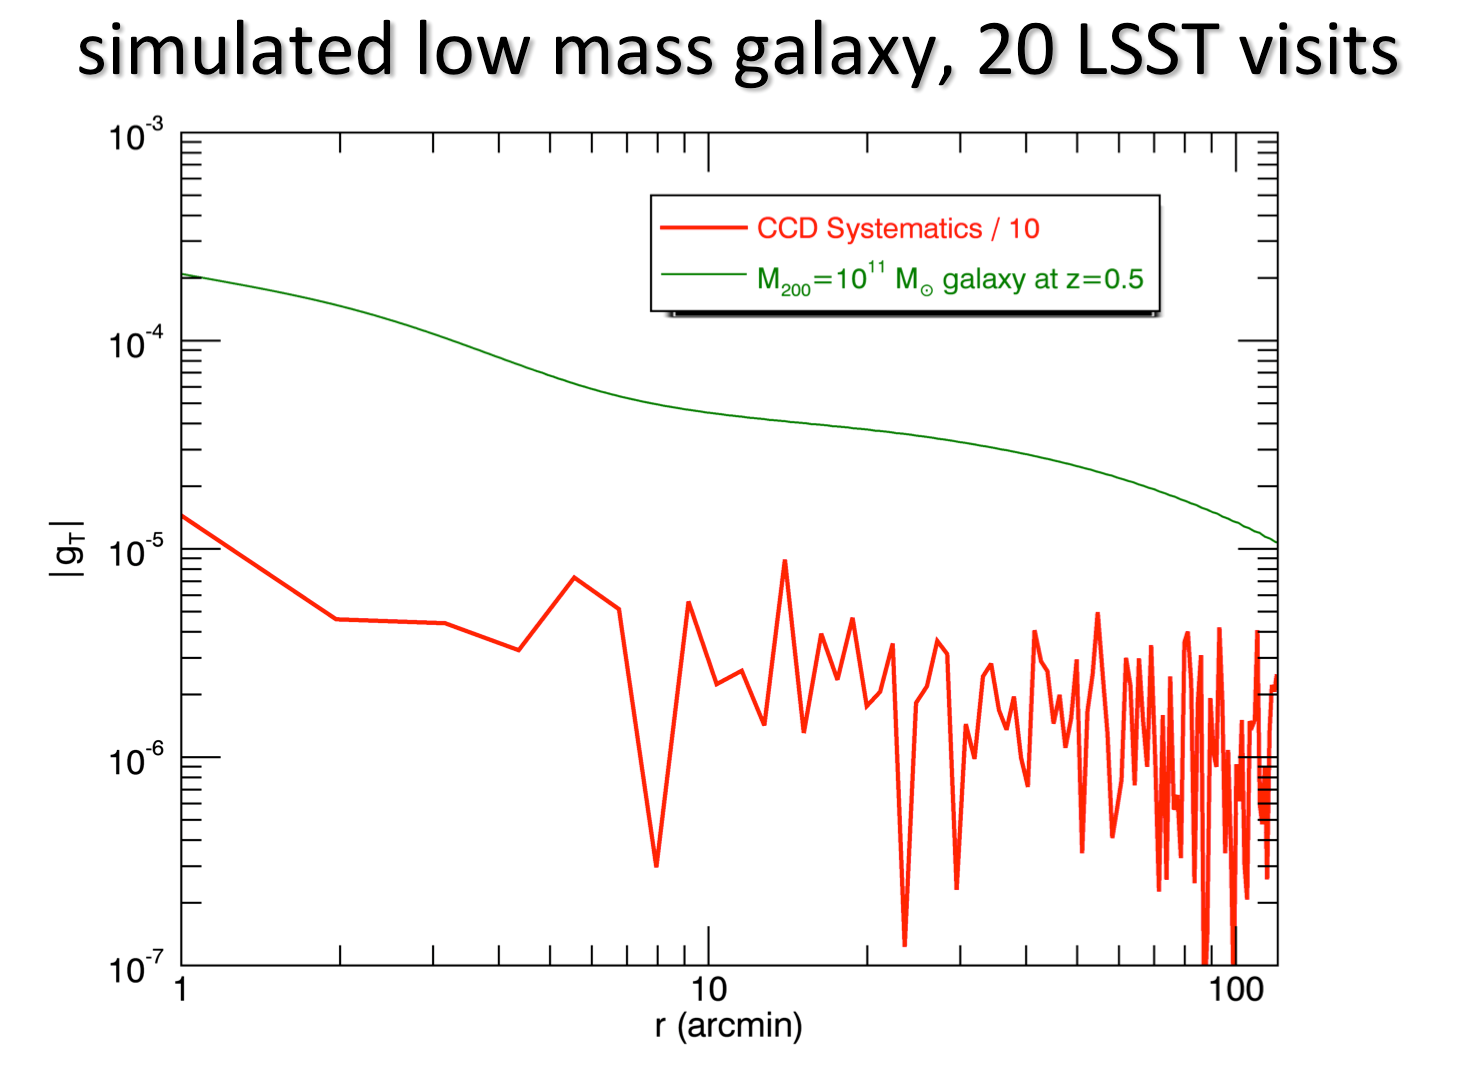
\includegraphics[width=0.6\columnwidth]{WL_of_dwarf.png}
\caption{\label{fig:psf_systematics} 
A variant of this figure showing the expected mass profile and noise for a sample of 100,000 dwarf galaxies of $M_{200} = 10^{8} M_\odot$ and each with 200 visits.}
\end{figure}

\begin{figure}
\centering
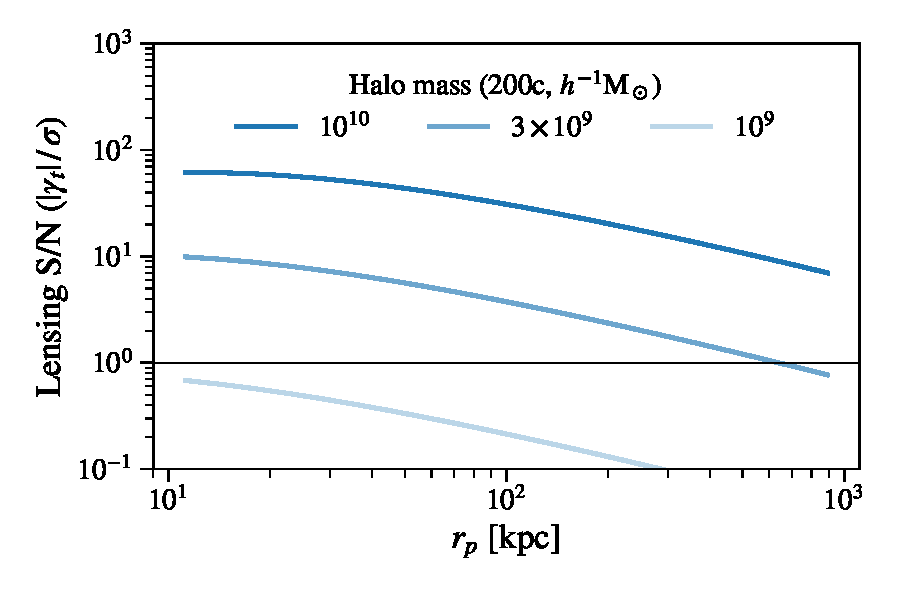
\includegraphics[width=0.7\columnwidth]{halo_mass_lensing_sn}
\caption{\label{fig:dwarf_sn} Lensing signal-to-noise for stacked samples of dwarf galaxies. 
This plot assumes perfect selection of dwarf galaxies within the redshift range over which they are detectable by LSST. 
Source galaxies are assumed to be at $z=1.2$, with a surface number density of $50 \amin^{-2}$, and a shear uncertainty of $\sigma_\gamma = 0.25$ per component.}
\end{figure}


\paragraph{Challenges} (observational, theoretical interpretation, etc.)

LSB galaxies are more likely to be removed from the catalog due to sky oversubtraction.

\paragraph{Going beyond dwarf galaxy detection limit.}
If we can stack on dwarf galaxies that are not detected in optical light of their stellar population, we can further extend our measurement to even lower mass regime. How can we find a faint galaxy whose surface brightness is below the noise level. We need a signpost unbiased to mass. One possible strategy is to stack image cutouts on SNe that are not near any detected galaxy. Potentially, they belong to very low-mass dwarf galaxies. This leverages the deep imaging and the time domain LSST data products. We do not require good SN light curves, so main survey WFD data is most relevant for discovery of the SN. We could then stack a large number of these, enabling optical detection of the stacked surface brightness as well as weak lensing mass profile measurement.  Some near-IR space imaging could help, as would sensitive SKA data.  Angular cross correlations of such a sample of dwarf galaxies with normal galaxies in the same redshift range could test evolutionary scenarios.
\end{comment}
